\subsection{Solution within the PEOM Method}\label{sec:sqd-peom}

In the PEOM method, we approximate the time-dependent dipole moment of the
MNP by
%
\begin{equation}
    \pmnp(t) \approx \sum_{k=1}^{N}c_k\real{s_k(t)} \ ,
    \label{eq:pmnpt_peom}
\end{equation}
%
where the functions, $\{s_k\}$, are found by solving the differential
equations,
%
\begin{equation}
    \dot{s}_k = -\left( \gamma_k + \imagn\omega_k \right)s_k + \imagn\epsb
    \emnp(t)\ \quad \text{for }k=1,2,\ldots,N \
    .
    \label{eq:s_k_mnp}
\end{equation}
%
The first step in the implementation, therefore, is to determine the paramters,
$\{c_k,\omega_k,\gamma_k\}$, by fitting the frequency-dependent
polarizability of the MNP, $\alphamnp(\omega)$, to
%
\begin{equation}
    \alphamnp(\omega) \approx \sum_{k=1}^{N}\frac{c_k}{2}
    \left[ \frac{1}{\omega+\omega_k +\imagn\gamma_k}
    -\frac{1}{ \omega-\omega_k +\imagn\gamma_k}\right] \ .
    \label{eq:alphamnp_approx}
\end{equation}
%
The polarizability
for the gold MNP from \cref{eq:alpha_mnp} is shown in \cref{fig:alpha_approx} along with a least-squares
fit to \cref{eq:alphamnp_approx} which required $N=$~\num{21} fitting functions in order to get a fit of
sufficient accuracy over the range \SIrange{0}{10}{\electronvolt}. The
parameters obtained are given in Appendix REF \note{Should I include these in
the appendix?}.

\begin{figure}[ht]
    \centering
    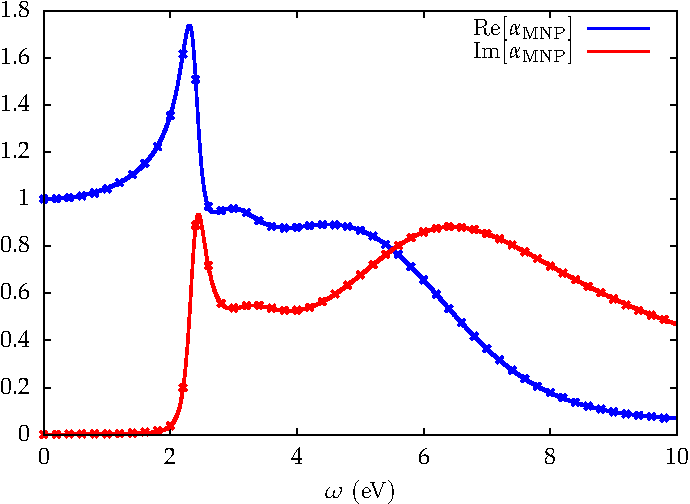
\includegraphics[width=0.8\textwidth]{alpha_mnp_approx.pdf}
    \caption{Real (solid blue) and imaginary (solid red) parts of the MNP
        frequency-dependent polarizability, $\alphamnp(\omega)$, as
        given by \cref{eq:alpha_mnp}. The least-squares fit is shown as
        crosses, obtained from \cref{eq:alphamnp_approx} with
        $N=$~\num{21}. The units of the $y$-axis are in $1/a^3$ where $a$ is the radius of
the MNP.}
    \label{fig:alpha_approx}
\end{figure}

Once the parameters are known, we can then solve \cref{eq:eoms} simultaneously
with \eqref{eq:s_k_mnp} using the fourth-order
Runge-Kutta method (\cref{app:runge-kutta}) where at the end of each step
$\pmnp(t)$ and $\psqd(t)$ are updated using \cref{eq:pmnpt_peom,eq:psqdt}
resepectively.  \note{(Should I include code/pseudo code of the algorithm in
the Appendix?)}.
